\documentclass[letterpaper, reqno,11pt]{article}
\usepackage[margin=1.0in]{geometry}
\usepackage{color,latexsym,amsmath,amssymb,graphicx, float}
\usepackage{hyperref}

\hypersetup{
colorlinks=true,
linkcolor=magenta,
filecolor=magenta,
urlcolor=cyan,
}

\graphicspath{ {images/} }

\begin{document}
\pagenumbering{arabic}
\title{ELEC 481 Homework 3}
\date{29/05/22}
\author{Xander Naumenko}
\maketitle


{\noindent\bf Question 1a.} 
\[
\text{EUAC}=A+S(A/F, i, n)=16500+12000(A /F, i, n)=\$19368
.\]

{\noindent\bf Question 1b.} 
\[
P=16500(P /A, 0.03, 4)+12000 / 1.03^{4}=\$71994
.\]

{\noindent\bf Question 1c.} 
\[
P=16500(P /A, 0.03, \infty)+12000 / (1.03^{4}-1)=\$645611
.\]

{\noindent\bf Question 2.} Total cost: 
\[
\text{EUAC}_A=A+P(A /P, i, n)-S (A/F, i, n)=\$2552
.\]
\[
\text{EUAC}_B=A+P(A /P, i, n)-S (A/F, i, n)=\$2692
.\]
Since the cost of machine A is lower than machine B, the company should use machine A. 

{\noindent\bf Question 3.} Putting the investment into excel, we arrive at a revenue stream as described in table \ref{fig:q3}. Using the excel IRR function we see that the annual rate of return is $3.5\%$. 

\begin{figure}[htpb]
    \centering
    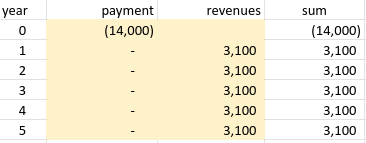
\includegraphics[width=0.8\textwidth]{q3}
    \caption{Revenue stream of question 3}
    \label{fig:q3}
\end{figure}

{\noindent\bf Question 4.} Since bonds don't compound, the revenue stream can be calculated as seen in figure \ref{fig:q4}. The yearly income was calculated simply as a percentage of the original bond's worth: 
\[
A=P\cdot i
.\]

\begin{figure}[htpb]
    \centering
    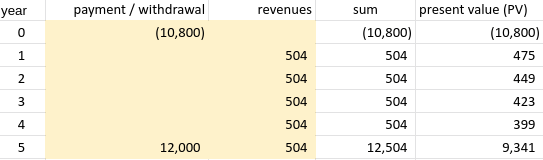
\includegraphics[width=0.8\textwidth]{q4}
    \caption{Revenue flow for question 4. }
    \label{fig:q4}
\end{figure}

Using the IRR function on the last column, we find that the annual effective interest rate is 6.6\%. 


{\noindent\bf Question 5.} To find the effective annual interest rate we have to compare the current option with the alternative, which is to pay by cash. Doing this results in a revenue stream as described in table \ref{fig:q5}. 

\begin{figure}[htpb]
    \centering
    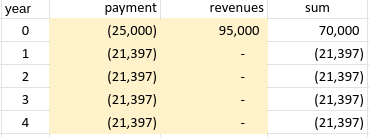
\includegraphics[width=0.8\textwidth]{q5}
    \caption{Revenue stream of question 5. }
    \label{fig:q5}
\end{figure}

Note that the \%95000 in revenue represents the incremental analysis of not doing the next best option, which is to buy the machine with cash. The yearly payments were calculated using the formula: 
 \[
A=P (A /P, i, n)
.\]
Applying the IRR function to the last column we find that the effective annual interest rate is 8.6\%. 

{\noindent\bf Question 6.} A plot of the EUAC of each option is shown in figure \ref{fig:q6}. These values were calculated in excel using the formula: 
\[
\text{EUAC}=A-P(A /P, i, n)
.\]

\begin{figure}[htpb]
    \centering
    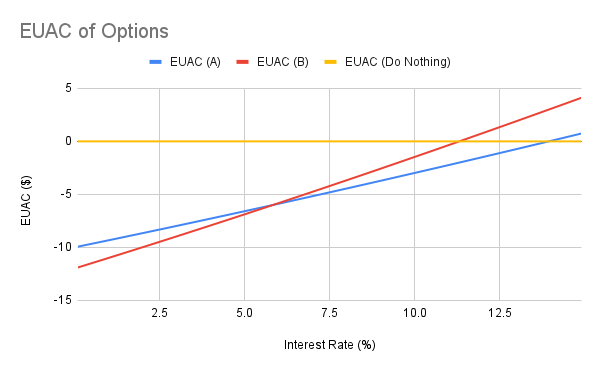
\includegraphics[width=0.8\textwidth]{q6.png}
    \caption{Graph of the EUAC for each option in question 6. }
    \label{fig:q6}
\end{figure}

From this graph we can find the option with the lowest EUAC for each interest rate, and we can make the table seen in table \ref{tab:q6}. 

\begin{table}[htpb]
    \centering
    \caption{Choice table for question 6. }
    \label{tab:q6}
    \begin{tabular}{c|c}
        Interest rate (\%)&Choice\\
        \hline\\
        Under 5.8&B\\
        5.8-11.3&A\\
        Over 11.3&Do Nothing

    \end{tabular}
\end{table}

\end{document}
